\subsection{Bidirectional Attentive Fusion with Context Gating for Dense Video Captioning}

\subsubsection{Overview}
Wang \textit{et al} propose to solve the Dense Video Captioning task by introducing a novel 
\textit{Bidirectional Single Stream Temporal Action Proposals} (Bi-SST) method for proposal 
generation. It utilizes both past and future video context while making event predictions, 
making use of \textit{context gating} to balance the contribution from current event 
proposal and the surrounding contexts dynamically. They identify the problem of inability of 
proposal generators to distinguish between events ending at around the same time (called 
\textit{discrimination property}) by \textit{attentive fusion} of hidden states of the 
proposal generator and the video features. During inference, a \textit{joint ranking} scheme 
is used to combine the proposal score and the caption confidence to get high confidence 
(proposal, caption) pairs \cite{wang2018bidirectional}.\par 


\subsubsection{Datasets}
\begin{itemize}
\item ActivityNet Captions \cite{krishna2017densecaptioning}
\item THUMOS-14 \cite{thumos-14} for proposals
\end{itemize}

\subsubsection{Performance}
\par 
Wang \textit{et al} report better performance on the ActivityNet Captions dataset with 
Bidirectional SST compared to the original SST in terms of the Meteor metric. For the task 
of Temporal Action Proposals, they report state of the art performance using the F1@1000 
metric on the THUMOS-14 dataset.
\par 
An ablation study investigates the effect of different mechanisms on the performance of their model:
\begin{itemize}
\item Bidirectional SST
\item Using hidden states of the LSTM (called \textit{context vectors}) for generating 
descriptions
\item Using the clipped video features corresponding to an event for caption generation
\item Temporal Dynamic Attention to fuse context vectors and clipped video features for 
caption generation
\item Context Gating
\item Joint Ranking
\end{itemize}
The results of this study reveals that the best model is the one which has all the 
aforementioned mechanisms / components in place.

\subsubsection{Methodology}

\begin{figure}[h]
	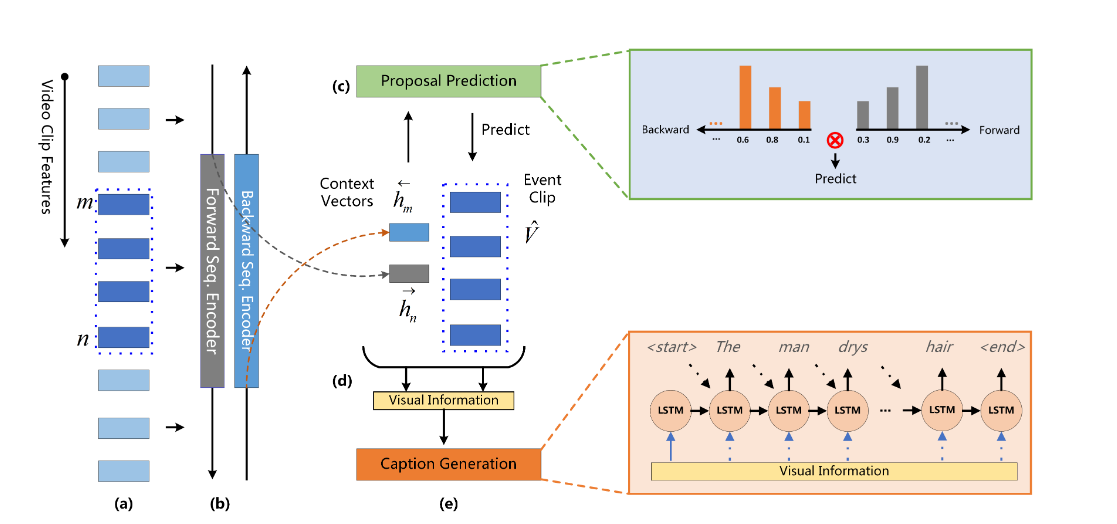
\includegraphics[width=\linewidth]{assets/img/bi-sst-architecture.png}
	\caption{Working of the Bidirectional SST (Image courtesy \cite{wang2018bidirectional})}
\end{figure}

\paragraph{Video input and preprocessing} 
	
\sloppy The video sequence is represented as a sequence of $L$ frames, $X = \{ x_1, x_2, x_3, ..., x_L \}$. Each video frame is encoded using a 3D CNN pre-trained on the Sports-1M dataset \cite{large-scale-video-classification-cnn}. 
Extracted C3D features have a temporal resolution of 16 frames, i.e., each feature vector 
corresponds to 16 frames. Principal Component Analysis (PCA) is then used to reduce feature 
dimensionality, giving the final visual stream: $V = \{v_1, v_2, v_3, ..., v_{L/16}\}$.

\paragraph{Proposal Module (Bi-SST)}
\begin{enumerate}
\item \textbf{Forward pass}: $V$ is input in forward order. The LSTM sequentially encodes 
the visual stream $V$, accumulating visual cues across time. The LSTM hidden states encode 
visual information in passed time steps. The hidden states of the LSTM are fed into $k$ 
independent binary classifiers (sigmoid activation, $0-1$), giving $k$ confidence scores. 
Each of these scores is of the proposal with end time as current time, and start time as $t 
- l_i$, where $\{l_1, l_2, l_3, ..., l_k\}$ are the lengths of the predefined $k$ proposal 
anchors.

\item\textbf{Backward pass}: $V$ is input in reverse order. The LSTM again encodes the 
visual stream, but in reverse order. The hidden states are fed to the $k$ classifiers, which 
predict their scores for $k$ proposals \textbf{starting} at current time. So as in 
the forward pass, we get $k$ proposals and their confidence at every time step.

\item\textbf{Fusion}: The two sets of proposals are fused by performing a Hadamard 
product of the confidence scores. This effectively combines past context (from forward pass), 
future context (from backward pass).

\item Proposals with scores larger than a specified threshold $\tau$ will be selected for 
captioning.

\item The training loss used is weighted multi-label cross entropy, averaged along time steps.
\end{enumerate}

\paragraph{Captioning Module}
For caption generation, if only the LSTM's hidden state from the proposal generator is taken 
as the input, the discrimination property of an event representation is not fulfilled. There 
can be at maximum $k$ proposals at every time step, but only one hidden state corresponds to 
that time step. Hence, to get a more discriminative event representation, the LSTM hidden 
state (context vectors) is fused with the corresponding visual features to help discriminate 
overlapping events, using Temporal Dynamic Attention, i.e., visual features are attended with 
respect to context vectors. Instead of simple concatenation of attended visual features and 
context vectors, a \textit{context gate} is used to balance their relative contribution. The 
motive behind this is that the network should learn how much context should be used to 
generate the next word. Finally, joint ranking is used to select high confidence (proposal, 
caption) pairs. Captioning loss is the sum of negative log likelihood of correct work in a 
sentence with $M$ words.



\subsubsection{Conclusion}
\par This paper introduced a novel proposal generator, Bi-SST which effectively encodes past 
as well as future context of the video to generate proposals. It also uses attentive fusion  
with context gating to combine, with weights, the proposal state  (context vectors) with 
visual features to generate captions and addresses the discriminative property problem. The 
joint ranking technique used is very intuitive as a confidence calculation method for dense 
captions.
